\documentclass[
    a4paper,
    11pt,
    parskip=half,   % Europäischer Absatzabstand
    ngerman         % Deutsche Silbentrennung
]{scrartcl}

% --- Pakete ---
\usepackage[utf8]{inputenc}
\usepackage[T1]{fontenc}
\usepackage{babel}
\usepackage{lmodern}            % Bessere Schriftart
\usepackage[margin=2.5cm]{geometry} 
\usepackage{graphicx}
\usepackage{xcolor}
\usepackage{tabularx}           % Flexible Tabellen
\usepackage{booktabs}           % Schöne Tabellenlinien
\usepackage{enumitem}           % Anpassbare Listen
\usepackage{tikz}               % Für Architektur-Diagramme
\usetikzlibrary{shapes.geometric, arrows, positioning, fit, calc}
\usepackage{hyperref}
\usepackage{amsmath}

% --- Farben (Konsistent mit D2.3) ---
\definecolor{hawblue}{RGB}{0, 51, 102}

% --- Metadaten ---
\title{\textbf{Deliverable D2.1: GEMS-Systemspezifikation \& Benchmarks}}
\subtitle{Projekt: PhyLFlex | Arbeitspaket 2.1}
\author{Verantwortlich: HAW Landshut (HAWL)}
\date{Version 1.0 (Entwurf)}

\begin{document}

\maketitle

% Projekt-Kopfdaten
\begin{description}[style=multiline, leftmargin=3.5cm, font=\bfseries]
    \item[Projekt:] PhyLFlex
    \item[Arbeitspaket:] AP 2.1 (Konzeptionierung eines netzdienlichen GEMS)
    \item[Partner:] TUM, ÜZW, SAG
\end{description}

\hrule
\tableofcontents
\vspace{1em}
\hrule
\vspace{1em}

% -------------------------------------------------------------------
\section{Kurzfassung}
Dieses Dokument dient als technisches \textbf{Lastenheft} für die Gebäude-Energie-Management-Systeme (GEMS), die in den Arbeitspaketen AP 4 (Konvex), AP 5 (RL) und AP 8 (Physikbasiert) entwickelt werden. 

Das System ist als kostengünstige Edge-Computing-Lösung definiert, die in der Lage ist, lokale Energieflüsse zu optimieren und gleichzeitig externe Signale des Verteilnetzbetreibers (VNB/DSO) einzuhalten.

% -------------------------------------------------------------------
\section{Hardware- \& Effizienz-Restriktionen}
Um die Skalierbarkeit über tausende von Haushalten zu gewährleisten, müssen die GEMS-Algorithmen für ressourcenbeschränkte Hardware ausgelegt sein. Die Entwicklung muss daher auf einen \textbf{Edge-Controller} abzielen.

\subsection{Referenz-Hardware}
\begin{table}[h]
\centering
\renewcommand{\arraystretch}{1.3} % Zeilenabstand etwas erhöhen
\begin{tabularx}{\textwidth}{lX}
\toprule
\textbf{Merkmal} & \textbf{Edge-Controller Spezifikation} \\
\midrule
\textbf{Gerätemodell} & Raspberry Pi 4 Model B (oder äquivalenter Industrie-Edge-PC) \\
\textbf{OS-Umgebung} & Linux (Dockerized Containers) \\
\textbf{Max. RAM-Nutzung} & $< 4\,\text{GB}$ \\
\textbf{Inferenzzeit} & $< 60\,\text{Sekunden}$ (pro 15-Min-Intervall) \\
\textbf{Leistungsaufnahme} & $< 6\,\text{Watt}$ \\
\bottomrule
\end{tabularx}
\caption{Hardware-Anforderungen für das GEMS}
\end{table}

\subsection{Funktionale Architektur}
Um die Vergleichbarkeit zwischen den verschiedenen algorithmischen Ansätzen (Konvex vs. RL) sicherzustellen, nutzt das System ein strikt modulares Design.

% TikZ Diagramm für die Architektur
\begin{figure}[h]
\centering
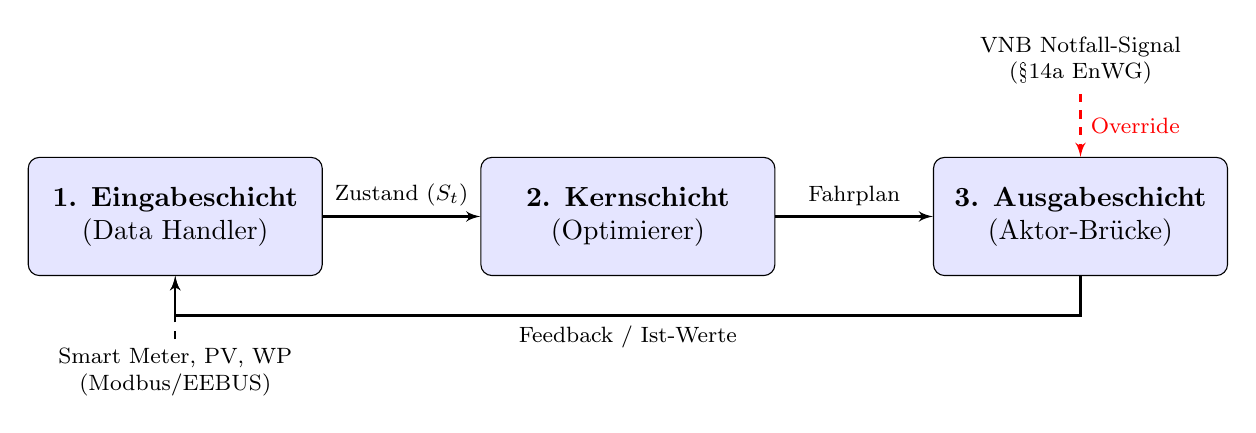
\begin{tikzpicture}[node distance=1.5cm, auto,
    block/.style={rectangle, draw, fill=blue!10, text width=3.5cm, text centered, rounded corners, minimum height=1.5cm},
    line/.style={draw, -latex', thick},
    cloud/.style={draw, ellipse, fill=red!10, node distance=3cm, minimum height=2em}]

    % Nodes
    \node [block] (input) {\textbf{1. Eingabeschicht}\\(Data Handler)};
    \node [block, right=2cm of input] (core) {\textbf{2. Kernschicht}\\(Optimierer)};
    \node [block, right=2cm of core] (output) {\textbf{3. Ausgabeschicht}\\(Aktor-Brücke)};
    
    % Externe Einflüsse
    \node [below=0.8cm of input, text width=3cm, align=center, font=\footnotesize] (devices) {Smart Meter, PV, WP\\(Modbus/EEBUS)};
    \node [above=0.8cm of output, text width=3cm, align=center, font=\footnotesize] (grid) {VNB Notfall-Signal\\(§14a EnWG)};

    % Paths
    \path [line] (input) -- node [font=\footnotesize] {Zustand ($S_t$)} (core);
    \path [line] (core) -- node [font=\footnotesize] {Fahrplan} (output);
    
    % Feedback Loop
    \path [line] (output.south) -- ++(0,-0.5) -| node [near start, below, font=\footnotesize] {Feedback / Ist-Werte} (input.south);
    
    % External connections
    \path [line, dashed] (devices) -- (input);
    \path [line, dashed, red] (grid) -- node [right, font=\footnotesize, red] {Override} (output);

\end{tikzpicture}
\caption{Abstrakte Modul-Architektur des GEMS}
\end{figure}

\begin{enumerate}
    \item \textbf{Eingabeschicht (Data Handler):} Aggregiert Daten von Smart-Meter-Gateways (iMSys), PV-Wechselrichtern und Wärmepumpen via Modbus/EEBUS. 
    \begin{itemize}
        \item Diese Schicht fungiert als lokale Datensenke.
        \item Hochfrequente Nutzerverhaltensdaten (1s-Auflösung) verbleiben im lokalen RAM und werden nicht exportiert, um \textbf{DSGVO-Konformität} zu gewährleisten.
    \end{itemize}

    \item \textbf{Kernschicht (Der Optimierer):} Dies ist das austauschbare Modul, in das AP 4, AP 5 und AP 8 ihre spezifischen Algorithmen integrieren.
    \begin{itemize}
        \item \textit{Eingabe:} Systemzustand (SoC, Temperatur, Prognose).
        \item \textit{Ausgabe:} Fahrplan (Control Schedule).
    \end{itemize}

    \item \textbf{Ausgabeschicht (Aktor-Brücke):} Übersetzt den Fahrplan in gerätespezifische Befehle.
    \begin{itemize}
        \item \textbf{Sicherheitsübersteuerung (Safety Override):} Drosselt Lasten sofort bei Empfang eines Notfallsignals gemäß §14a EnWG (Umgehung des Optimierers).
        \item \textbf{Zustandsrückführung (Feedback):} Meldet tatsächliche Leistungswerte zurück an die Kernschicht, um Zustandsschätzer (z.\,B. Batterie-SoC) zu aktualisieren.
    \end{itemize}
\end{enumerate}

\newpage

% -------------------------------------------------------------------
\section{Definition der Testfälle (Szenarien)}
Es werden vier standardisierte Szenarien definiert, um das GEMS zu evaluieren. Diese Szenarien decken die Zielkonflikte zwischen Nutzerautonomie und Netzstabilität ab.

\subsection{Szenario A: Der Insel-Optimierer (Baseline)}
\begin{itemize}
    \item \textbf{Fokus:} Autarkie (Eigenversorgung).
    \item \textbf{Beschreibung:} Das GEMS optimiert rein auf die Maximierung des PV-Eigenverbrauchs. Es findet keine externe Kommunikation mit dem Netz oder Nachbarn statt.
    \item \textbf{Zweck:} Dient als Basislinie (Baseline) zur Bewertung von Effizienzgewinnen in komplexeren Szenarien.
\end{itemize}

\subsection{Szenario B: Die P2P-Community}
\begin{itemize}
    \item \textbf{Fokus:} Lokales Energy Sharing.
    \item \textbf{Beschreibung:} Gebäude tauschen Daten bezüglich überschüssiger Erzeugung aus. Haus A (PV-Überschuss) teilt virtuell Energie mit Haus B (Wärmepumpen-Bedarf).
    \item \textbf{Metrik:} Reduktion des gesamten Community-Imports/-Exports am Transformatorpunkt.
\end{itemize}

\subsection{Szenario C: Netzorientierter Betrieb (§14a EnWG)}
\begin{itemize}
    \item \textbf{Fokus:} Netzstabilität \& Compliance.
    \item \textbf{Beschreibung:} Der VNB sendet eine dynamische Leistungsgrenze (z.\,B. „Max. Bezug: $4,2\,\text{kW}$“) an das GEMS. Das System muss flexible Lasten (EVs, Wärmepumpen) drosseln, während unflexible Lasten (Beleuchtung, Kochen) weiterlaufen.
    \item \textbf{Erfolgskriterium:} Keine Verletzungen des Leistungsgrenzwert-Signals (Hard Constraint).
\end{itemize}

\subsection{Szenario D: Preisgesteuerter Betrieb (§41a EnWG)}
\begin{itemize}
    \item \textbf{Fokus:} Wirtschaftliche Optimierung.
    \item \textbf{Beschreibung:} Das GEMS empfängt dynamische Strompreise (z.\,B. Spotmarkt oder Time-of-Use-Tarife). Es verschiebt große Lasten in günstige Stunden.
    \item \textbf{Risiko-Analyse:} Bewertung von Synchronisationseffekten (Lawineneffekt), bei denen sich alle Haushalte gleichzeitig einschalten und potenziell neue Netzengpässe verursachen.
\end{itemize}

\end{document}